\documentclass[a4paper]{article}

% Packages
\usepackage[margin = 1 in]{geometry}
\usepackage{fancyhdr}
\usepackage{lastpage}
\usepackage{ctex}
\usepackage[utf8]{inputenc} % Required for inputting international characters
\usepackage[english]{babel}
\usepackage[T1]{fontenc} % Output font encoding for international characters
\usepackage[sfdefault]{ClearSans} % Use the Clear Sans font (sans serif)
\usepackage{graphicx}
\usepackage{caption}
\usepackage{subcaption}
\usepackage{float}
\usepackage{amsmath}
\usepackage{amsfonts}
\usepackage{enumitem}
\usepackage{hyperref}
\usepackage{titlesec}
\usepackage{lipsum}
\usepackage{geometry}
\usepackage{tocloft} 

\pagestyle{fancy}
% Formatting
\geometry{margin=1in}
\setlength{\parindent}{0pt}
\setlength{\parskip}{1em}
\renewcommand{\baselinestretch}{1.5}
\renewcommand{\cftsecleader}{\cftdotfill{\cftdotsep}}
\rhead{\thepage}

% Title and Author
\title{\textbf{Challenges and Strategies for Sentiment Analysis of Irony and Humor in Social Media Based on Machine Learning}}
\author{Zijun Li}
\date{\today}

% Document
\begin{document}
\setlength{\parindent}{2em}

% Title Page
\maketitle
\thispagestyle{empty}

%% Abstract
\begin{abstract}
    Sentiment analysis of irony and humor in social media poses a formidable challenge owing to the complexity and context-dependency of such expressions. This report offers a comprehensive overview of diverse machine learning techniques utilized in the analysis of irony and humor, encompassing traditional machine learning algorithms and deep learning approaches. We explore the practical implementation of these techniques by examining specific examples and assess the challenges and future prospects of sentiment analysis concerning irony and humor in social media.
\end{abstract}

% Table of Contents
% \newpage
% \tableofcontents
% \thispagestyle{empty}

% Introduction
\newpage
\setcounter{page}{1}
\section{Introduction}

The rapidly growing popularity of social media platforms has necessitated understanding user sentiment through text for various applications, including marketing, customer service, and opinion mining. Irony and humor, prevalent in social media, pose significant challenges for sentiment analysis due to their context-dependency, diverse forms, and intricate language features.

As science and technology advance, artificial intelligence increasingly permeates from specialized domains into everyday life. The Verta Insights Study reveals that among investment strategies across six distinct spending categories for 2022 and 2023, the AI innovation technology category remains the top priority, with 54\% and 58\% of respondents ranking it as such, respectively. This underscores the importance of artificial intelligence technology in social development.

Given the rising significance of artificial intelligence and the challenges presented by irony and humor in sentiment analysis, this review aims to offer a comprehensive overview of methods and strategies to address sentiment analysis of irony and humor in social media using machine learning techniques. We commence by defining irony and humor, expounding on their complexities within the social media context. Following that, we explore various machine learning strategies, their practical implementations, and the advantages and limitations of each method. Finally, we delve into the challenges and future directions for this research area, emphasizing the necessity for ongoing innovation and enhancement in techniques to better comprehend and analyze sentiment in social media text.

% irony and Humor in Sentiment Analysis
\section{The basic concepts of irony and humor sentiment analysis}

Prior to exploring machine learning methods for analyzing irony and humor in sentiment analysis, it is crucial to establish a clear understanding of the definitions of irony and humor. This will facilitate better classification and labeling of data for analysis.

\subsection{The concepts of Irony}

Irony is a rhetorical device that involves a discrepancy between what is expected and what actually occurs, or between the intended meaning and the literal meaning of words. It is commonly used in literature, language, and everyday conversation to create humor, emphasize a point, or express subtle criticism. Among the various types of irony, verbal irony and situational irony are the most common.\cite{ref_concept1,ref_concept2}

\begin{itemize}
\item {\bf Verbal irony} occurs when a speaker's intended meaning is opposite or contrary to the literal meaning of their words. For instance: 
    \subitem \textit{"Oh, great! Just what I needed—a flat tire!"} 
    \\The speaker's words seem to express enthusiasm, but their actual intention is to convey frustration or disappointment about the flat tire.
\item {\bf Situational irony} arises when there is a discrepancy between the expected outcome of a situation and the actual outcome. This type of irony is often used to create a dramatic effect, add depth to a story, or convey a moral lesson, featuring prominently in literature. For example:
    \subitem \textit{In Shakespeare's Romeo and Juliet, the two lovers plan to elope and live happily ever after. However, their pursuit of happiness ultimately leads to their tragic demise.}
\end{itemize}

\subsection{The concepts of Humor}

Humor is a multifaceted and subjective concept, often defined as a form of communication that elicits laughter and entertainment, typically prompted by unexpected or incongruous situations. 
Humor can be verbal, visual, or physical. In this discussion, we will concentrate on verbal humor, which can be further classified into the following categories:\cite{ref_concept1}

\begin{itemize}
    \item {\bf Self-irony}: Referring to self-irony, frequently employed to defuse tense situations or alleviate embarrassment. Example:
        \subitem\textit{"I hate it when I go to hug someone really sexy and my face smashes right into the mirror."}
        \\Using self-irony to indicate that the "someone sexy" is the speaker.
    \item {\bf Exaggeration/Hyperbole}: Utilizing extreme exaggeration to emphasize a point or add humor. Example:
        \subitem\textit{"I'm so hungry, I could eat a horse!"}
        \\Normally, a human cannot eat an entire horse. The extreme exaggeration is used to convey the speaker's intense hunger.
    \item {\bf Phonetics Assisted}: Generating humor by manipulating phonetic and pronunciation features. The production of this humor usually depends on the syllables, rhythm, and intonation of the language. Example:
        \subitem\textit{"I'm reading a book on the history of glue – I just can't seem to put it down."}
        \\The double meaning of the phrase "put it down" is employed because it can refer to physically placing a book down and stopping reading a book.
    \item {\bf Semantic Opposites}: Using words with opposite meanings to create a humorous effect. Example:
        \subitem\textit{"I love sleeping, it's like being dead without the commitment."}
        \\This example underscores the speaker's love for sleeping by using the contrasting idea of death without its finality.
    \item {\bf Secondary Meaning}: A word or phrase with multiple meanings, used to create a humorous effect. Example:
        \subitem\textit{"Why do we tell actors to 'break a leg'? Because every play has a cast."}
        \\In this example, the phrase "break a leg" possesses a secondary meaning in the theater world as a way of wishing someone good luck before a performance, even though the literal meaning is negative.
\end{itemize}

% Machine Learning-based Strategies for Sentiment Analysis of irony and Humor in Social Media
\section{machine learning strategy for sentiment analysis of irony and humor}

After comprehending the fundamental classification of irony and humor, it is crucial to collect data sets, preprocess the data, extract features, and train various models to achieve recognition. Machine learning-based sentiment analysis methods are typically classified into traditional machine learning and deep learning approaches. This section explores traditional machine learning methods, such as Support Vector Machines (SVM), Decision Trees, Random Forests, and Naive Bayes Classifier, as well as deep learning models, including Convolutional Neural Networks (CNN), Recurrent Neural Networks (RNN), Transformers, among others. These techniques are analyzed to determine their efficacy in sentiment analysis tasks related to irony and humor.

\subsection{Machine learning algorithms}

Machine learning algorithms, a subset of artificial intelligence, enable machines to learn and enhance their performance from experience without explicit programming. These algorithms are extensively employed in sentiment analysis, including the analysis of irony and humor.

In sentiment analysis of irony and humor, feature engineering is a prevalent approach where relevant features, such as sentiment words, part-of-speech tags, and syntactic patterns, are identified and employed to train the classifier. For instance, detecting the presence of positive or negative sentiment words in a text can aid in classifying humor, while recognizing ironic expressions like understatement or overstatement can be utilized to classify irony.

Another approach involves ensemble methods, which integrate multiple classifiers to enhance the accuracy of the analysis. For example, combining decision trees and support vector machines (SVMs) could be employed to classify text as humorous or non-humorous. Ensemble methods have demonstrated improved performance in sentiment analysis of irony and humor compared to individual classifiers.

\subsubsection{Support Vector Machines, SVM}

\textbf{Support Vector Machines(SVM)} is a supervised learning algorithm commonly used for classification and regression tasks. The core principle of SVM is to divide the dataset into distinct categories by identifying an optimal hyperplane. In the case of binary classification, SVM aims to find a hyperplane during training that maximizes the margin between the two different categories, effectively partitioning the data.

The Decision function is known as$$f(x) = w^T \phi(x) + b$$
\begin{itemize}
    \item $f(x)$: the output of the decision function, indicating the classification of the input sample $x$
    \item $w$: the weight vector, which is learned during training and used to make classifications
    \item $\phi(x)$: the feature vector that represents the input sample $x$. This feature vector is derived from the original data using a transformation function.
    \item $b$: the bias term, which shifts the decision boundary away from the origin. It is also learned during training.
\end{itemize}

When the dataset is linearly separable, SVM identifies a unique hyperplane that separates the data into two classes. However, if the dataset is not linearly separable, SVM employs a technique called kernel function to transform the data from the original space to a higher-dimensional space, where the data becomes linearly separable.\cite{ref_svm1}

\begin{figure}[H]
    \centering
    \begin{minipage}{0.48\textwidth}
      \centering
      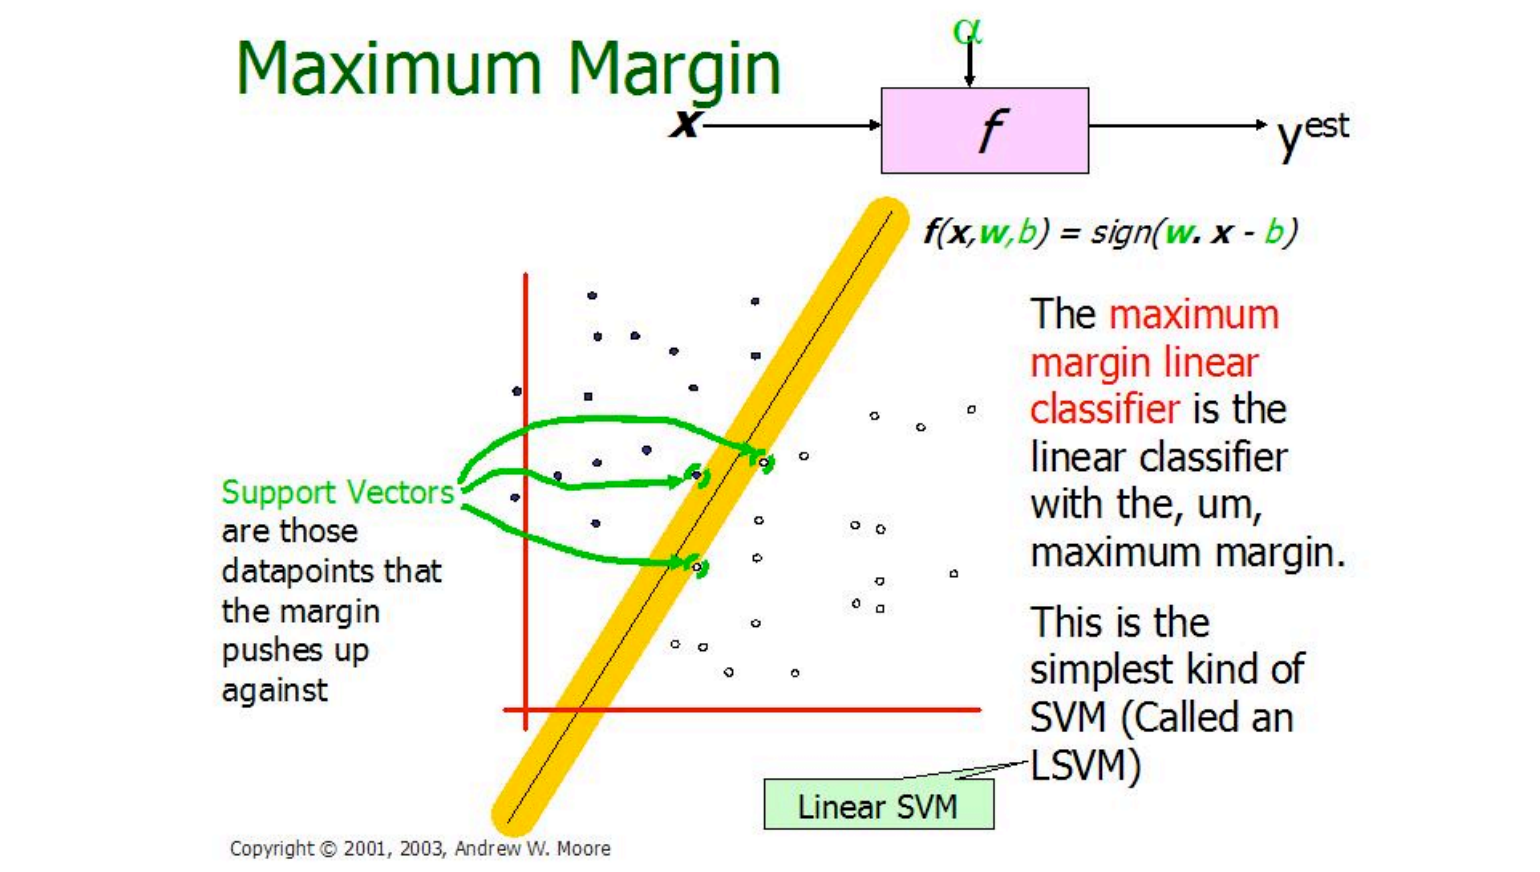
\includegraphics[width=\linewidth]{./images/SVM_Linear SVM.png}
      \caption{SVM: Linear SVM}
      \label{fig.SVM_Linear SVM[Illustration of Linear SVM. (Taken from Andrew W. Moore slides 2003)]}
    \end{minipage}\hfill
    \begin{minipage}{0.48\textwidth}
      \centering
      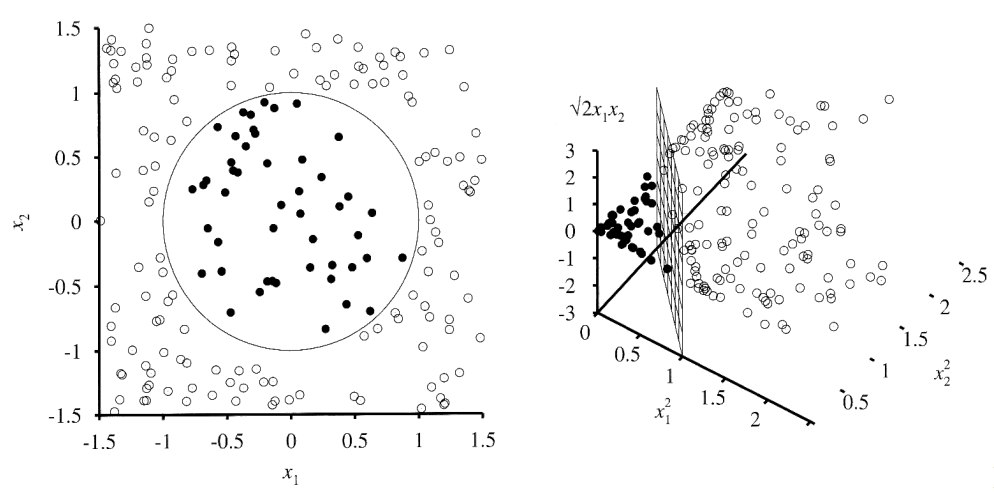
\includegraphics[width=\linewidth]{./images/SVM_High-dimensional_Space.png}
      \caption{SVM: Mapping data into a high-dimensional space\cite{ref_svm2}}
      \label{fig.SVM_High-dimensional_Space}
    \end{minipage}
\end{figure}

The selection of appropriate parameters is critical for achieving effective performance and generalization capabilities when training an SVM for sentiment analysis. Different combinations of parameters can have a significant impact on the model's performance. In this regard, two important SVM parameters are explained below:
\begin{itemize}
    \item \textbf{Kernel function}: The selection of an appropriate kernel function is vital to achieve optimal SVM performance. For datasets that are linearly separable, a linear kernel function typically results in better classification outcomes. However, for nonlinear datasets, polynomial and Radial Basis Function (RBF) kernels are commonly used. Polynomial kernels can capture polynomial relationships, while RBF kernels can handle complex nonlinear relationships. Different kernel functions can be compared using cross-validation during the selection process.\cite{ref_svm1}
    \item \textbf{C}: C is a regularization parameter in SVM, and its value is an important factor in the objective function, which can be expressed as $$\min_{w, b} \frac{1}{2} |w|^2 + C \sum_{i=1}^n \xi_i$$A larger value of C implies a greater penalty for misclassification, increasing the risk of overfitting. On the other hand, a smaller value of C indicates a lower penalty for misclassification, which heightens the risk of underfitting. In practice, various values of C can be tested, and the optimal value is typically found using cross-validation on a logarithmic scale. \cite{ref_svm3}
\end{itemize}

\subsubsection{Decision Trees \& Random Forests}

\textbf{A decision tree} is a tree-structured classification algorithm that partitions the dataset, with each internal node representing a feature and each leaf node representing a category. The decision tree is built recursively, selecting each node based on a specific characteristic, typically using information gain or the Gini index. Information gain measures a feature's importance for classification, while the Gini index measures the purity of samples.

During the decision tree's classification process, starting from the root node, input samples are categorized according to the characteristics represented by each node, then assigned to corresponding child nodes until reaching the leaf nodes. Each leaf node represents a category, and the sample is ultimately assigned to a specific leaf node, which constitutes the sample's classification result.\cite{ref_dt2}

\begin{figure}[H]
    \centering
    \begin{minipage}{0.48\textwidth}
      \centering
      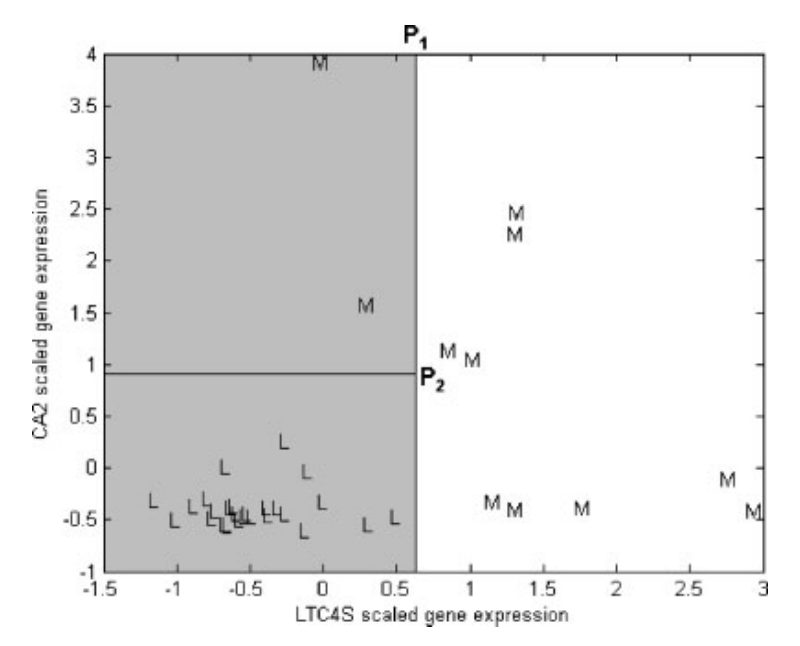
\includegraphics[width=\linewidth]{./images/Decision tree-Recursively-partitioned feature space.png}
      \caption{Decision tree: Recursively-partitioned feature space (features 1 and 2) of $X_T$.\cite{ref_dt1}}
      \label{fig.Decision tree-data}
    \end{minipage}\hfill
    \begin{minipage}{0.48\textwidth}
      \centering
      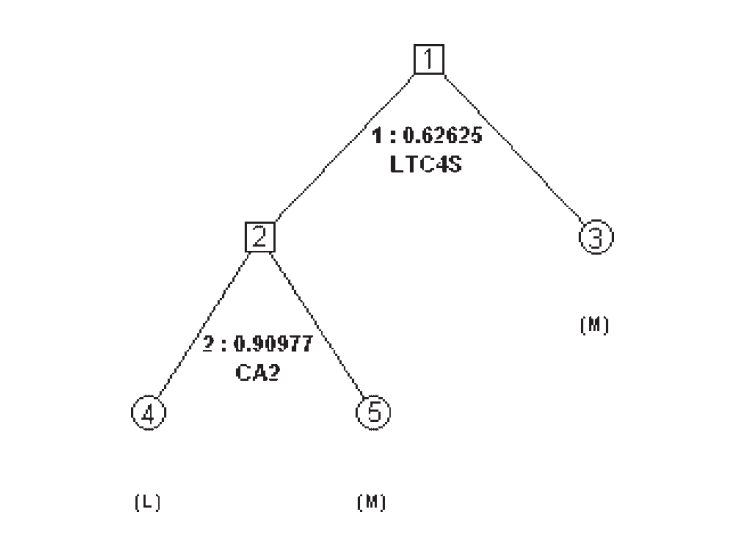
\includegraphics[width=\linewidth]{./images/Decision tree.png}
      \caption{Decision tree: Decision tree corresponding to the partitioned feature space in Figure 3.\cite{ref_dt1}}
      \label{fig.Decision tree}
    \end{minipage}
\end{figure}

To prevent overfitting, the decision tree undergoes continuous pruning during training based on the training data. Pruning is generally divided into two methods: pre-pruning and post-pruning. \cite{ref_dt3}Pre-pruning limits each node's division during tree construction to avoid overfitting, while post-pruning trims a complete tree after establishment to reduce overfitting. 

\textbf{Random Forests} is an ensemble learning method that enhances classification or regression accuracy by constructing multiple decision trees. Each decision tree is obtained by randomly subsampling the training data and training with a random subset of features. At testing time, each decision tree classifies or regresses the input data, and the results from all decision trees are integrated to produce a final prediction.

We use the random forest algorithm to train the training set, generating multiple decision trees. At each decision tree node, we select a feature to classify and divide the dataset into two subsets. This process repeats until specific conditions are met.

\subsubsection{Naive Bayes Classifier}

The Naive Bayes classifier is a machine learning algorithm based on Bayes' theorem, which assumes feature independence, meaning the values of each feature under a given category are independent.

Specifically, the Naive Bayes classifier transforms a text data sentiment classification problem into a conditional probability calculation. Given text data $D$, the probability $P(c|D)$ of it belonging to a certain sentiment category $c$ must be calculated. According to Bayes' theorem, $P(c|D)$ can be expressed as:

$$P(c|D)=\dfrac{P(D|c)P(c)}{P(D)}$$

Here, $P(D|c)$ denotes the probability of text data $D$ occurring under the given emotion category $c$; $P(c)$ represents the probability of emotion category $c$ occurring; and $P(D)$ is the probability of text data $D$ occurring. As $P(D)$ is identical for all sentiment categories, it can be disregarded.\cite{ref_nbc1}

The Naive Bayes classifier presumes that for a given class $c$, the values of each feature $x_i$ are independent. Thus, the conditional probability $P(D|c)$ can be expressed as:

$$P(D|c)=P(x_1|c) \times P(x_2|c) \times ... \times P(x_n|c)$$

Here, $x_1, x_2, ..., x_n$ represent the features of text data $D$, and $n$ is the number of features.\cite{ref_nbc1}

In the study conducted by Ankur Goel, Jyoti Gautam, and Sitesh Kumar\cite{ref_nbc2}, the authors propose a method that combines SentiWordNet and Naive Bayes to enhance the accuracy of sentiment analysis for tweets. SentiWordNet is a sentiment lexicon that assigns sentiment scores to words, reflecting their positivity, negativity, and objectivity. The findings demonstrate that incorporating SentiWordNet with the Naive Bayes classifier can lead to improved sentiment analysis accuracy.

% \subsubsection{Summary}
% 
% \begin{table}[ht]
%     \centering
%     \renewcommand{\arraystretch}{1.2}
%     \resizebox{\textwidth}{!}{%
%     \footnotesize
%     \begin{tabular}{|p{3cm}|p{5cm}|p{5cm}|p{2cm}|p{3cm}|}
%     \hline
%     Model & Advantages & Disadvantages & Use Cases & Applications \\ \hline
%     Support Vector Machines & Effective in high-dimensional spaces, \newline robust to outliers, \newline maximizes margin between classes & May not perform well on large datasets, \newline sensitive to choice of kernel & Text classification, \newline image classification, \newline regression & Sentiment analysis, \newline handwriting recognition, \newline bioinformatics \\ \hline
%     Decision Trees \newline and Random Forests & Easy to interpret, \newline can handle mixed data types, \newline scalable to large datasets (Random Forests) & May be prone to overfitting (Decision Trees), \newline can be complex and computationally expensive (Random Forests) & Classification, \newline regression, \newline feature selection & Customer segmentation, \newline fraud detection, \newline medical diagnosis \\ \hline
%     Naive Bayes Classifier & Easy to implement, \newline computationally efficient, \newline handles missing data & Assumes feature independence, \newline may not perform well when features are correlated & Text classification, \newline spam filtering, \newline sentiment analysis & Sentiment analysis, \newline document classification, \newline spam detection \\ \hline
%     \end{tabular}%
%     }
%     \resizebox{\textwidth}{!}{%
%     \footnotesize
%     \begin{tabular}{|p{3cm}|p{7cm}|p{8cm}|}
%     \hline
%     Model & Input Data & Key Formulas \\ \hline
%     Support Vector Machines & Input: $X \in \mathbb{R}^{n \times d}$ (feature matrix), \newline Labels: $y \in {-1, 1}^n$ (class labels) & Decision function: $f(x) = w^T \phi(x) + b$,\newline Objective: $\min_{w, b} \frac{1}{2} |w|^2 + C \sum_{i=1}^n \xi_i$, \newline Constraint: $y_i (w^T \phi(x_i) + b) \geq 1 - \xi_i, \xi_i \geq 0$ \\ \hline
%     Decision Trees \newline and Random Forests & Input: $X \in \mathbb{R}^{n \times d}$ (feature matrix), \newline Labels: $y \in \mathbb{R}^n$ (class labels or continuous target) & Decision Tree: $y = f(x)$,\newline Random Forest: $y = \frac{1}{B} \sum_{b=1}^B f_b(x)$, \newline where $f_b(x)$ is a decision tree \\ \hline
%     Naive Bayes Classifier & Input: $X \in \mathbb{R}^{n \times d}$ (feature matrix), \newline Labels: $y \in \mathbb{R}^n$ (class labels) & Conditional probability: $P(c|D) = \frac{P(D|c) P(c)}{P(D)}$, \newline Naive assumption: $P(D|c) = P(x_1|c) \times P(x_2|c) \times \cdots \times P(x_n|c)$ \\ \hline
% \end{tabular}%
% }
% \end{table}

\subsection{Deep learning algorithm}

Deep learning algorithms have demonstrated considerable potential in numerous natural language processing tasks, encompassing sentiment analysis of irony and humor. This section explores prominent deep learning methods, including Convolutional Neural Networks (CNNs), Recurrent Neural Networks (RNNs), Long Short-Term Memory (LSTM) networks, and Transformers, and their applications in irony and humor analysis tasks.

\subsubsection{Convolutional Neural Networks (CNNs)}

Although CNNs are predominantly utilized in image processing, they can also be employed for text classification tasks, including irony and humor analysis. They operate by applying convolutional filters to extract features from text and pooling layers to diminish the dimensionality of the extracted features.

The application of CNNs in humor and irony sentiment analysis hinges on convolution and pooling operations. Convolution operations capture local features in the text, while pooling operations reduce feature dimensions and enhance feature robustness. CNNs accept text input as a matrix, convolve it with multiple convolution kernels, and then use pooling operations for feature extraction and dimensionality reduction. Ultimately, a fully connected layer classifies the features.  \cite{ref_cnn2}

\begin{figure}[H]
    \centering
    \begin{minipage}{0.48\textwidth}
      \centering
      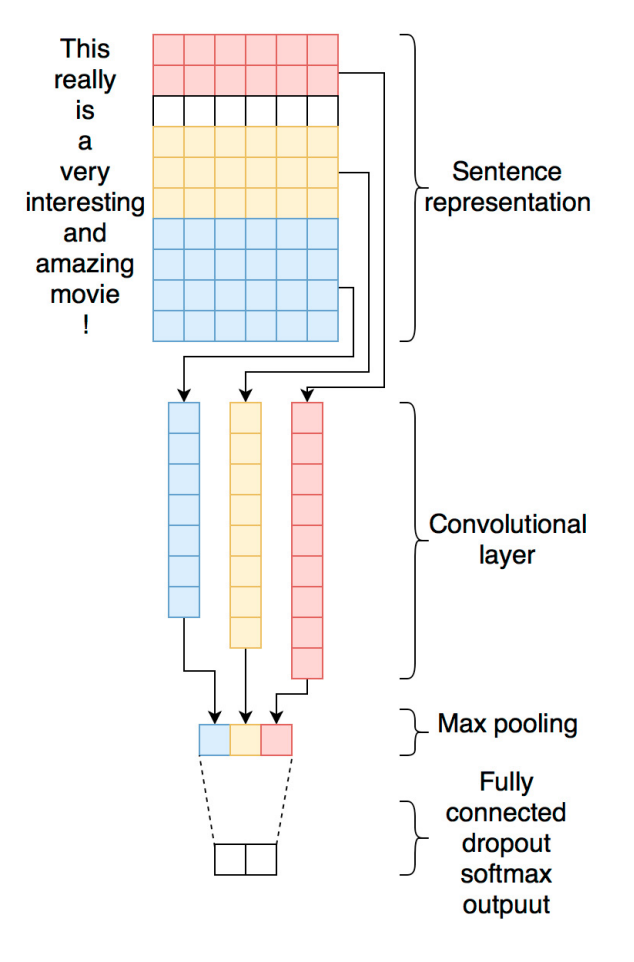
\includegraphics[width=\linewidth]{./images/CNN_architecture.png}
      \caption{CNN: Example architecture \cite{ref_cnn1}}
      \label{fig.CNN_1}
    \end{minipage}\hfill
    \begin{minipage}{0.48\textwidth}
        The training process of CNNs entails the following steps:
        \begin{enumerate}
            \item Input layer: The input layer receives the text data for analysis.
            \item Convolutional layer: This layer applies a set of filters to the input data to detect specific features, such as word sequences, patterns, and structures.
            \item Pooling layer: The pooling layer downsamples the activation layer's output by summarizing the information in neighboring activations.
            \item Fully connected layer: This layer takes the pooling layer's output and applies a set of weights to generate a final output.
            \item Output layer: The output layer yields a probability distribution over possible sentiment labels (e.g., positive, negative, ironic, humorous).
        \end{enumerate}
    \end{minipage}
\end{figure}

\begin{figure}
    \centering
    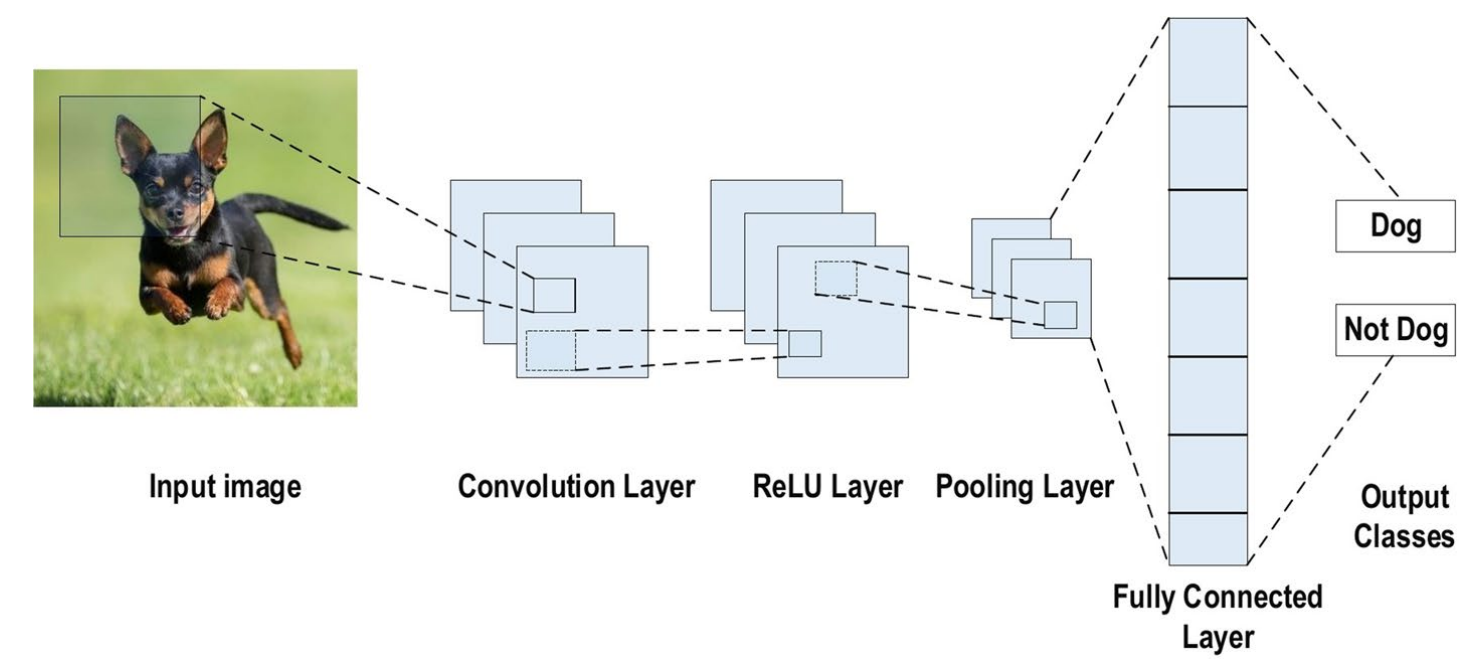
\includegraphics[width=0.8\linewidth]{./images/CNN_architecture_2.png}
    \caption{CNN in Image recognition}
    \label{fig.CNN_2}
\end{figure}

\subsubsection{Recurrent Neural Networks (RNNs)}

Recurrent Neural Networks (RNNs) constitute another deep learning algorithm suitable for humor and irony sentiment analysis. RNNs excel at analyzing sequential data, crucial for comprehending the context of humorous or ironic statements.

\begin{figure}[H]
    \centering
    \begin{minipage}{0.48\textwidth}
        \centering
        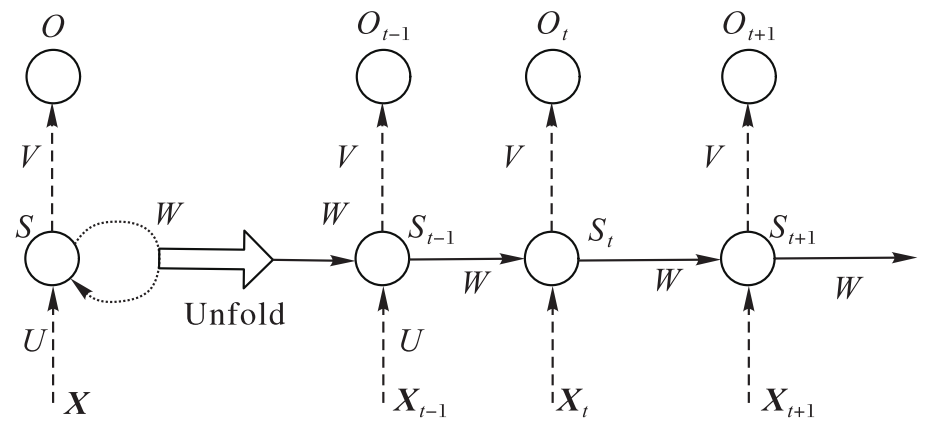
\includegraphics[width=1\textwidth]{./images/RNN_architecture.png}
        \caption{RNN: Example architecture \cite{ref_rnn1}}
        \label{fig.RNN}
    \end{minipage}\hfill
    \begin{minipage}{0.48\textwidth}
        The fundamental principle of RNNs involves using the output from a previous time step as input to the current time step, enabling the network to maintain a form of memory for previous inputs. This feature is especially beneficial for analyzing text sequences, where a word or phrase's meaning may rely on the context of preceding text.
    \end{minipage}
\end{figure}

A significant application of RNNs in humor and irony analysis involves generating new text that is humorous or ironic. By training an RNN on a dataset of humorous or ironic text, the model can learn to generate new text that mirrors the style and tone.

\paragraph{Long Short-Term Memory (LSTM)}

Long Short-Term Memory (LSTM) represents a specialized RNN model designed for processing sequential data and has gained widespread use in irony and humor sentiment analysis.

\begin{figure}[H]
    \centering
    \begin{minipage}{0.48\textwidth}
        \centering
        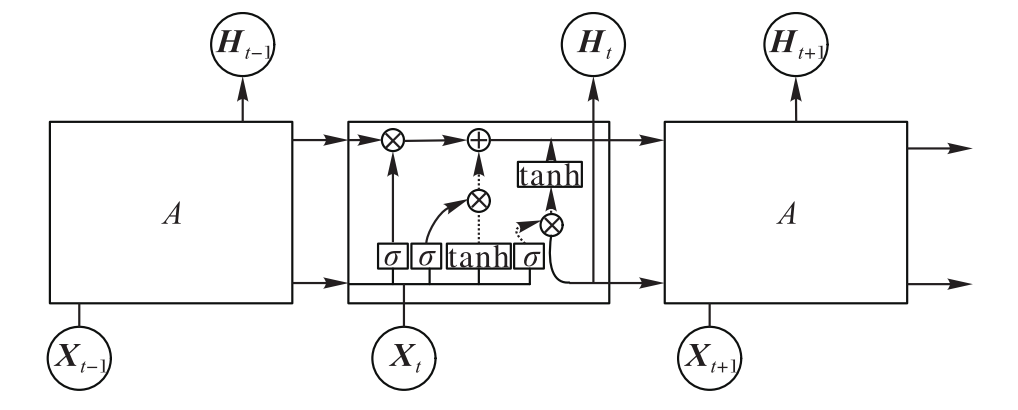
\includegraphics[width=1\textwidth]{./images/LSTM_architecture.png}
        \caption{LSTM: Example architecture \cite{ref_rnn1}}
        \label{fig.LSTM}
    \end{minipage}\hfill
    \begin{minipage}{0.48\textwidth}
        In contrast to traditional RNN models, LSTM incorporates three gate mechanisms: input, forget, and output gates. These gates control the influence of information passed from previous moments and current moment input on subsequent moments. This mechanism effectively addresses the vanishing gradient problem associated with long sequence data, thereby enhancing the model's performance.
    \end{minipage}
\end{figure}

In humor and irony sentiment analysis, LSTMs frequently model text sequences to capture contextual and semantic information within language. By learning long-term dependencies, LSTMs gain a better understanding of implicit semantics and logic in humor and irony, leading to improved sentiment analysis.

LSTM models typically require extensive data for training to achieve optimal performance. During the training process, the backpropagation algorithm updates the model's parameters, while techniques such as cross-validation evaluate the model's performance and generalization capabilities. Ultimately, the trained model performs sentiment analysis on new text data, classifying and recognizing humor and irony.

In the study conducted by Krupa Patel, Manasi Mathkar, Sarjak Maniar, Avi Mehta, and Shachi Natu, the researchers presented a comprehensive approach for employing an LSTM (Long Short-Term Memory) model to detect humor in text. The model achieved an impressive accuracy of 94.62\%.\cite{ref_rnn3}

\paragraph{AttBiLSTM (Attention-based Bidirectional Long Short-Term Memory)}

AttBiLSTM (Attention-based Bidirectional Long Short-Term Memory) extends the LSTM model by incorporating an additional attention mechanism and bidirectionality.

\begin{figure}[H]
    \centering
    \begin{minipage}{0.48\textwidth}
        \centering
        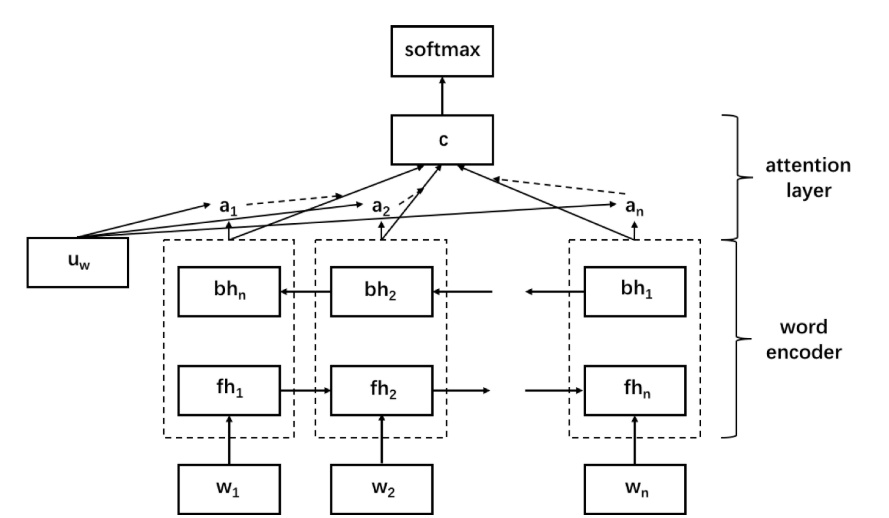
\includegraphics[width=1\textwidth]{./images/AttBiLSTM_architecture.png}
        \caption{AttBiLSTM:  architecture \cite{ref_rnn2}}
        \label{fig.AttBiLSTM}
    \end{minipage}\hfill
    \begin{minipage}{0.48\textwidth}
        In AttBiLSTM, a reverse LSTM processes the reverse part of the sequence at each time step, in addition to the forward LSTM. Furthermore, AttBiLSTM employs an attention mechanism to calculate the importance of each time step in the sequence, assigning importance to the corresponding hidden state to better capture key information within the sequence.
    \end{minipage}
\end{figure}

Compared to LSTM, AttBiLSTM offers superior sequence modeling and expressive capabilities, handles long sequences more effectively, and demonstrates higher performance in numerous natural language processing tasks.

\subsubsection{Transformers}

Transformers represent a neural network model based on the self-attention mechanism, originally proposed by Google. The core concept involves acquiring a comprehensive feature representation of the input sequence by executing self-attention weighted aggregation on the features of all positions within the input sequence.

Transformers generally comprise two stages: pre-training and fine-tuning. During the pre-training stage, the model learns to represent text data from a vast text corpus. In the fine-tuning stage, the model undergoes refinement on specific humor and irony datasets, enhancing its sentiment analysis capabilities for humor and irony. Distinct from traditional RNNs and CNNs, Transformers consider the semantics of the entire sentence when processing text, resulting in superior performance for humor and irony that require an understanding of contextual language forms.

% \subsubsection{Summary}
% 
% \begin{table}[ht]
%     \centering
%     \renewcommand{\arraystretch}{1.2}
%     \resizebox{\textwidth}{!}{%
%     \footnotesize
%     \begin{tabular}{|p{1.5cm}|p{5cm}|p{5cm}|p{3cm}|p{3cm}|}
%         \hline
%         Model & Advantages & Disadvantages & Use Cases & Applications \\ \hline
%         CNN & Good at capturing local dependencies, \newline efficient computation for parallel processing & May not capture long-term dependencies, \newline not suitable for variable-length input & Text classification, \newline object recognition, \newline image processing & Sentiment analysis, \newline image classification, \newline speech recognition \\ \hline
%         RNN & Can handle sequential data, \newline can capture long-term dependencies & May suffer from vanishing/exploding gradients, \newline computationally expensive & Language modeling, \newline speech recognition, \newline machine translation & Text generation, \newline speech synthesis, \newline handwriting recognition \\ \hline
%         LSTM & Addresses vanishing/exploding gradient problem, \newline can capture long-term dependencies & Computationally expensive, \newline not suitable for parallel processing & Speech recognition, \newline machine translation, \newline handwriting recognition & Text generation, \newline speech synthesis, \newline video processing \\ \hline
%         AttBiLSTM & Handles sequential data with attention mechanism, \newline captures both local and global dependencies & Computationally expensive, \newline may require large amounts of training data & Sentiment analysis, \newline language modeling, \newline machine translation & Text classification, \newline sentiment analysis, \newline chatbots \\ \hline
%         Transformer & Enables parallel processing, \newline can handle long-term dependencies & May require a large amount of training data, \newline less effective for real-time sequential data & Machine translation, \newline language modeling, \newline text generation & Chatbots, \newline text classification, \newline sentiment analysis \\ \hline
%     \end{tabular}%
%     }
%     \resizebox{\textwidth}{!}{%
%     \footnotesize
%     \begin{tabular}{|p{1.5cm}|p{10cm}|p{6cm}|}
%         \hline
%         Model & Input Data & Key Formulas \\ \hline
%         CNN & Input: $X \in \mathbb{R}^{W \times H \times C}$ (image or time-series data),\newline Weights: $W \in \mathbb{R}^{w \times h \times C \times N}$ (convolutional kernel) & Convolution: $Y_{i} = f(X * W_{i} + b_{i})$ \\ \hline
%         RNN & Input: $x_t \in \mathbb{R}^n$ (input at time step $t$),\newline Hidden state: $h_t \in \mathbb{R}^m$ (hidden state at time step $t$) & $h_t = f(W_{hh}h_{t-1} + W_{xh}x_t + b_h)$ \\ \hline
%         LSTM & Input: $x_t \in \mathbb{R}^n$ (input at time step $t$),\newline Hidden state: $h_t \in \mathbb{R}^m$ (hidden state at time step $t$),\newline Cell state: $c_t \in \mathbb{R}^m$ (cell state at time step $t$) & $\begin{aligned}
%             f_t &= \sigma(W_f[h_{t-1}, x_t] + b_f) \\
%             i_t &= \sigma(W_i[h_{t-1}, x_t] + b_i) \\
%             \tilde{c}_t &= \tanh(W_c[h_{t-1}, x_t] + b_c) \\
%             c_t &= f_t \odot c_{t-1} + i_t \odot \tilde{c}_t \\
%             o_t &= \sigma(W_o[h_{t-1}, x_t] + b_o) \\
%             h_t &= o_t \odot \tanh(c_t)
%         \end{aligned}$ \\ \hline
%         AttBiLSTM & Input: $x_t \in \mathbb{R}^n$ (input at time step $t$),\newline Hidden state: $h_t \in \mathbb{R}^m$ (hidden state at time step $t$),\newline Attention weights: $\alpha_{ij}$ (attention weight for input $j$ at time step $i$) & $\begin{aligned}
%             h_t^f &= \text{LSTM}_f(x_t, h_{t-1}^f) \\
%             h_t^b &= \text{LSTM}_b(x_t, h_{t+1}^b) \\
%             e_{ij} &= \text{score}(h_i^f, h_j^b) \\
%             \alpha_{ij} &= \frac{\exp(e_{ij})}{\sum_{k=1}^T \exp(e_{ik})} \\
%             c_i &= \sum_{j=1}^T \alpha_{ij} h_j^b \\
%             h_i &= \text{tanh}(W_c[h_i^f; c_i]) \\
%             \end{aligned}$ \\
%             \hline
%             Transformer & Input: $x \in \mathbb{R}^{T \times d_{\text{model}}}$ (sequence of embeddings),\newline Key, Query, Value: $K, Q, V \in \mathbb{R}^{T \times d_k}$ & $\begin{aligned}
%             Z &= \text{Self-Attention}(Q, K, V) \\
%             Z &= \text{LayerNorm}(x + Z) \\
%             F &= \text{FeedForward}(Z) \\
%             F &= \text{LayerNorm}(Z + F)\\
%         \end{aligned}$ \\
%         \hline
%     \end{tabular}%
%     }
% \end{table}

\section{Actual case analysis}

Upon examining the analysis of humor and irony using machine learning techniques, it is essential to adhere to a systematic process to achieve precise recognition. This process can be broadly divided into three principal steps:
\begin{enumerate}
    \item \textbf{Data Collection and Preprocessing}: The initial step involves gathering a diverse and representative dataset from the target domain. Once the dataset is obtained, preprocessing it is crucial, which entails removing irrelevant or redundant information, rectifying spelling errors, and converting the data into a format suitable for analysis.
    \item \textbf{Feature Extraction}: The subsequent step comprises extracting meaningful features from the preprocessed data, which can be utilized for training models. The selection of appropriate features is vital as it directly influences the models' performance. Various techniques can be employed for feature extraction, including bag-of-words, word embeddings, and other advanced natural language processing methods.
    \item \textbf{Model Training and Evaluation}: The concluding step entails training different models using the extracted features and evaluating their performance on the test dataset. This step involves selecting suitable models, tuning their hyperparameters, and testing their performance using various evaluation metrics such as accuracy, precision, recall, and F1 score.
\end{enumerate} 

\paragraph{HEMOS: A Novel Deep Learning-Based Fine-Grained Humor Detection Method for Sentiment Analysis of Social Media}\cite{ref_rnn2}

\subparagraph{Concepts}In a study conducted by Da Li, Rafal Rzepka, Michal Ptaszynski, and Kenji Araki, the researchers employed both lexicons and an \textbf{AttBiLSTM recurrent neural network} for sentiment analysis of Chinese social media, resulting in the creation of the HEMOS system.

\begin{figure}[H]
    \centering
    \begin{minipage}{0.48\textwidth}
        \centering
        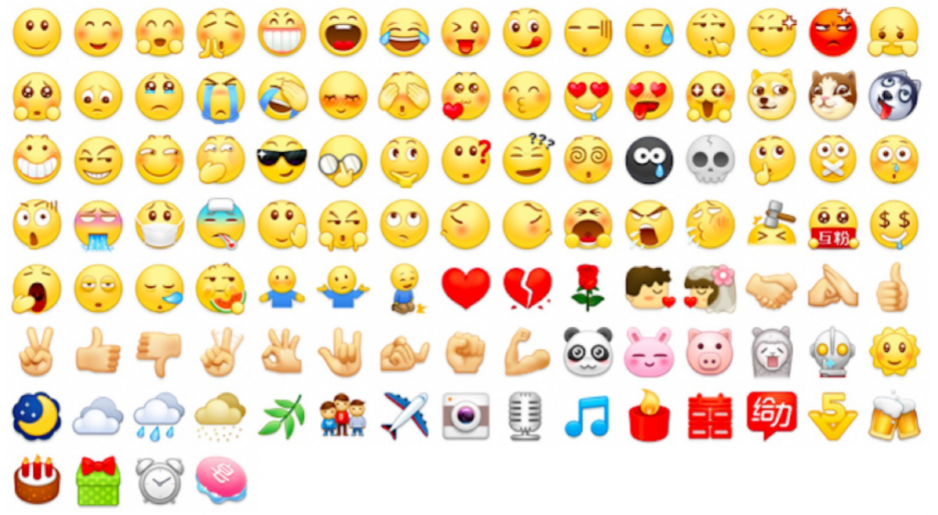
\includegraphics[width=1\textwidth]{./images/108_Weibo_emojis.png}
        \caption{109 Weibo emojis that can be transformed into Chinese character tags\cite{ref_rnn2}}
        \label{fig.109 Weibo emojis that can be transformed into Chinese character tags.}
    \end{minipage}\hfill
    \begin{minipage}{0.48\textwidth}
        Since emotions are often expressed through body language, and in social networks, this nonverbal communication can be partially mimicked by employing emojis and slang. The researchers combined emoticons, slang, and text to analyze whether Weibo action comments contained humor.
    \end{minipage}
\end{figure}

Based on these emojis and slang, various meanings were assigned to different emojis and slang as one criterion for assessing humor. This approach facilitated a more nuanced understanding of the content analyzed and enhanced the accuracy of sentiment analysis.

\subparagraph{Data Collection and Preprocessing \& Feature Extraction}The authors conducted research on sentiment analysis of Chinese social media, specifically focusing on detecting irony and humor in Weibo posts. They crawled a vast dataset of 7.6 million Weibo posts, filtered out images and videos, and trained word embeddings using the word2vec model. Additionally, they incorporated Chinese Internet slang and emoji lexicons into the dictionary of Jieba, a Chinese text segmentation package, to improve the accuracy of the text preprocessing stage.

\subparagraph{Model Training and Evaluation}To train their proposed model, the researchers collected 4000 Weibo posts containing ambiguous emojis and requested three Chinese native speakers to annotate them using four category labels: positive, negative, optimistic humorous, and pessimistic humorous. The AttBiLSTM model was subsequently trained with 10 epochs using a dropout rate of 0.25 and a batch size of 64, with the model's validity examined via 10-fold cross-validation.

\subparagraph{Test and Result}The authors tested the proposed model using a test set of 180 Weibo entries with eight specific emojis, comparing the results with and without considering Internet slang and emoji lexicons for both two-category sentiment classification (positive and negative) and four-category sentiment classification (positive, negative, optimistic humorous, and pessimistic humorous).

The findings revealed that the proposed model achieved superior performance in humor detection and sentiment analysis when considering Internet slang and emoji lexicons, even with small-scale data labeling. Notably, adding Internet slang and emoji lexicons enhanced the accuracy of identifying humorous entries, which are difficult to polarize. Moreover, the authors demonstrated that including "optimistic humorous" and "pessimistic humorous" categories improved the prediction of bi-polarity sentiment.

% Challenges of Sentiment Analysis of irony and Humor in Social Media

\section{Challenges of Sentiment Analysis for Irony and Humor}
Sentiment analysis of irony and humor in social media poses several challenges that render it a demanding task. Some of these challenges encompass:

\begin{itemize}
\item \textbf{Context-dependency}: Irony and humor often hinge on specific contexts and background knowledge for accurate comprehension and interpretation. Absent such context, the genuine sentiment of a text might be overlooked or misconstrued.
\item \textbf{Diversity}: Irony and humor can manifest in various forms, such as sarcasm, puns, and hyperbole. This diversity complicates the development of a comprehensive approach to sentiment analysis.
\item \textbf{Language features}: Irony and humor may entail intricate language features, including wordplay, ambiguity, and rhetorical devices. These features can pose challenges to detection and analysis using conventional NLP techniques.
\item \textbf{Cross-cultural differences}: Irony and humor may differ across cultures, complicating the development of models that function across diverse languages and cultural contexts.
\end{itemize}

% Future Directions and Outlook
\section{Future Directions and Outlook}
Several potential avenues for future research in sentiment analysis of irony and humor in social media include:

\begin{itemize}
\item \textbf{Cross-lingual and cross-cultural analysis}: Developing models capable of effectively detecting irony and humor across various languages and cultural backgrounds remains an ongoing challenge. Future research should concentrate on creating models that can address cross-lingual and cross-cultural disparities in humor and irony.
\item \textbf{Multimodal information fusion}: Incorporating multimodal features, such as images and videos, can enhance the accuracy of humor and irony detection models. Future research should aim to develop models that can efficiently integrate information from multiple modalities.
\item \textbf{Automatic discovery of new patterns}: Developing unsupervised or weakly supervised methods for automatically discovering novel patterns and expressions of irony and humor would constitute a substantial contribution to the field.
\item \textbf{Adversarial training}: Adversarial training can bolster the robustness and generalization of models for sentiment analysis of irony and humor. Future research should examine the efficacy of adversarial training in this context.
\item \textbf{Explainability and interpretability}: Enhancing the explainability and interpretability of sentiment analysis models for irony and humor is essential for fostering trust and comprehension. Future research should prioritize developing models that can deliver interpretable and transparent results.
\end{itemize}

\section{Conclusion}
In this report, we have investigated various machine learning strategies for sentiment analysis of irony and humor in social media, encompassing supervised learning, unsupervised learning, and deep learning approaches. Despite advances in these techniques, significant challenges persist in detecting and analyzing irony and humor, including context-dependency, diversity, language features, and cross-cultural differences. As we look ahead, promising research areas include cross-lingual and cross-cultural analysis, multimodal information fusion, automatic discovery of new patterns, adversarial training, and model explainability and interpretability. Tackling these challenges and pursuing these future directions will enable more accurate and robust sentiment analysis of irony and humor in social media.

\begin{thebibliography}{}
    \bibitem{ref_concept1}
    Reyes, A., Rosso, P., \& Buscaldi, D. (2012). From humor recognition to irony detection: The figurative language of social media. Data \& Knowledge Engineering, 74, 1–12. https://doi.org/10.1016/j.datak.2012.02.005
    \bibitem{ref_concept2}
    Barbieri, F., \& Saggion, H. (2014). Modelling Irony in Twitter (pp. 56–64). Association for Computational Linguistics. https://aclanthology.org/E14-3007.pdf
    \bibitem{ref_svm1}
    Mustafa Abdullah, D., \& Mohsin Abdulazeez, A. (2021). Machine Learning Applications based on SVM Classification A Review. Qubahan Academic Journal, 1(2), 81–90. https://doi.org/10.48161/qaj.v1n2a50
    \bibitem{ref_svm2}
    Gavrilov, Z. (n.d.). SVM Tutorial. https://web.mit.edu/zoya/www/SVM.pdf
    \bibitem{ref_svm3}
    Jordaan, E. M., \& Smits, G. F. (2002, May 1). Estimation of the regularization parameter for support vector regression. IEEE Xplore. https://doi.org/10.1109/IJCNN.2002.1007481
    \bibitem{ref_dt1}
    Myles, A. J., Feudale, R. N., Liu, Y., Woody, N. A., \& Brown, S. D. (2004). An introduction to decision tree modeling. Journal of Chemometrics, 18(6), 275–285. https://doi.org/10.1002/cem.873
    \bibitem{ref_dt2}
    Somvanshi, M., Chavan, P., Tambade, S., \& Shinde, S. V. (2016, August 1). A review of machine learning techniques using decision tree and support vector machine. IEEE Xplore. https://doi.org/10.1109/ICCUBEA.2016.7860040
    \bibitem{ref_dt3}
    Esposito, F., Malerba, D., Semeraro, G., \& Kay, J. (1997). A comparative analysis of methods for pruning decision trees. IEEE Transactions on Pattern Analysis and Machine Intelligence, 19(5), 476–493. https://doi.org/10.1109/34.589207
    \bibitem{ref_nbc1}
    Kaur, G., \& Er. Neelam Oberai. (2014). A REVIEW ARTICLE ON NAIVE BAYES CLASSIFIER WITH VARIOUS SMOOTHING TECHNIQUES. https://www.semanticscholar.org/paper/A-REVIEW-ARTICLE-ON-NAIVE-BAYES-CLASSIFIER-WITH-Kaur-Oberai/1c41b7b724e1245201c895160fb46cdd84dca809
    \bibitem{ref_nbc2}
    Goel, A., Gautam, J., \& Kumar, S. (2016, October 1). Real time sentiment analysis of tweets using Naive Bayes. IEEE Xplore. https://doi.org/10.1109/NGCT.2016.7877424
    \bibitem{ref_cnn1}
    Liao, S., Wang, J., Yu, R., Sato, K., \& Cheng, Z. (2017). CNN for situations understanding based on sentiment analysis of twitter data. Procedia Computer Science, 111, 376–381. https://doi.org/10.1016/j.procs.2017.06.037
    \bibitem{ref_cnn2}
    Alzubaidi, L., Zhang, J., Humaidi, A. J., Al-Dujaili, A., Duan, Y., Al-Shamma, O., Santamaría, J., Fadhel, M. A., Al-Amidie, M., \& Farhan, L. (2021). Review of deep learning: concepts, CNN architectures, challenges, applications, future directions. Journal of Big Data, 8(1). https://doi.org/10.1186/s40537-021-00444-8
    \bibitem{ref_rnn1}
    Wang, Y., Zhu, J., Wang, Z., Bai, F., \& Gong, J. (2022). Review of applications of natural language processing in text sentiment analysis. Journal of Computer Applications, 42(4), 1011. https://doi.org/10.11772/j.issn.1001-9081.2021071262
    \bibitem{ref_rnn2}
    Li, D., Rzepka, R., Ptaszynski, M., \& Araki, K. (2020). HEMOS: A novel deep learning-based fine-grained humor detecting method for sentiment analysis of social media. Information Processing \& Management, 57(6), 102290. https://doi.org/10.1016/j.ipm.2020.102290
    \bibitem{ref_rnn3}
    To laugh or not to laugh – LSTM based humor detection approach. (n.d.). Ieeexplore.ieee.org. Retrieved April 23, 2023, from https://ieeexplore.ieee.org/abstract/document/9580124
    \bibitem{ref_case1}
    Zhang, S., Zhang, X., Chan, J., \& Rosso, P. (2019). Irony detection via sentiment-based transfer learning. Information Processing \& Management, 56(5), 1633–1644. https://doi.org/10.1016/j.ipm.2019.04.006
    \bibitem{ref_case2}
    Troussas, C., Virvou, M., Espinosa, K. J., Llaguno, K., \& Caro, J. (2013). Sentiment analysis of Facebook statuses using Naive Bayes classifier for language learning. IISA 2013. https://doi.org/10.1109/iisa.2013.6623713
    \bibitem{ref_case3}
    Sykora, M., Elayan, S., \& Jackson, T. W. (2020). A qualitative analysis of sarcasm, irony and related \#hashtags on Twitter. Big Data \& Society, 7(2), 205395172097273. https://doi.org/10.1177/2053951720972735
\end{thebibliography}

\end{document}

